% !TeX spellcheck = pl_PL
\newpage
\part{\huge \textbf{Treść zadania}}
	\indent \indent \textit{Shoot' em up} (w skrócie zwany shmup) jest gatunkiem gier akcji wywodzącym się w prostej linii od gier typu \textit{Space Invaders} lub \textit{River Raid}. Kontrolowana przez gracza postać (np. statek) w pojedynkę stawia czoło przeciwnikom, niszcząc ich za pomocą wystrzeliwanych pocisków, jednocześnie unikając ich ataków. Podgatunek shmupów, zwany \textit{danmaku} (z jap. \textit{ściana pocisków} lub \textit{piekło pocisków}) kładzie większy nacisk na omijanie wrogich ataków, niż na ofensywie. Przykładowymi danmaku są np. \textit{Ikaruga} czy większość gier z uniwersum \textit{Touhou Project}. \\

	Gra powstała jako projekt łączony z przedmiotów \textit{Projekt Programistyczny} i \textit{Grafika Komputerowa} oraz miała spełniać następujące założenia:
	
	\begin{center}
		\fbox{%
			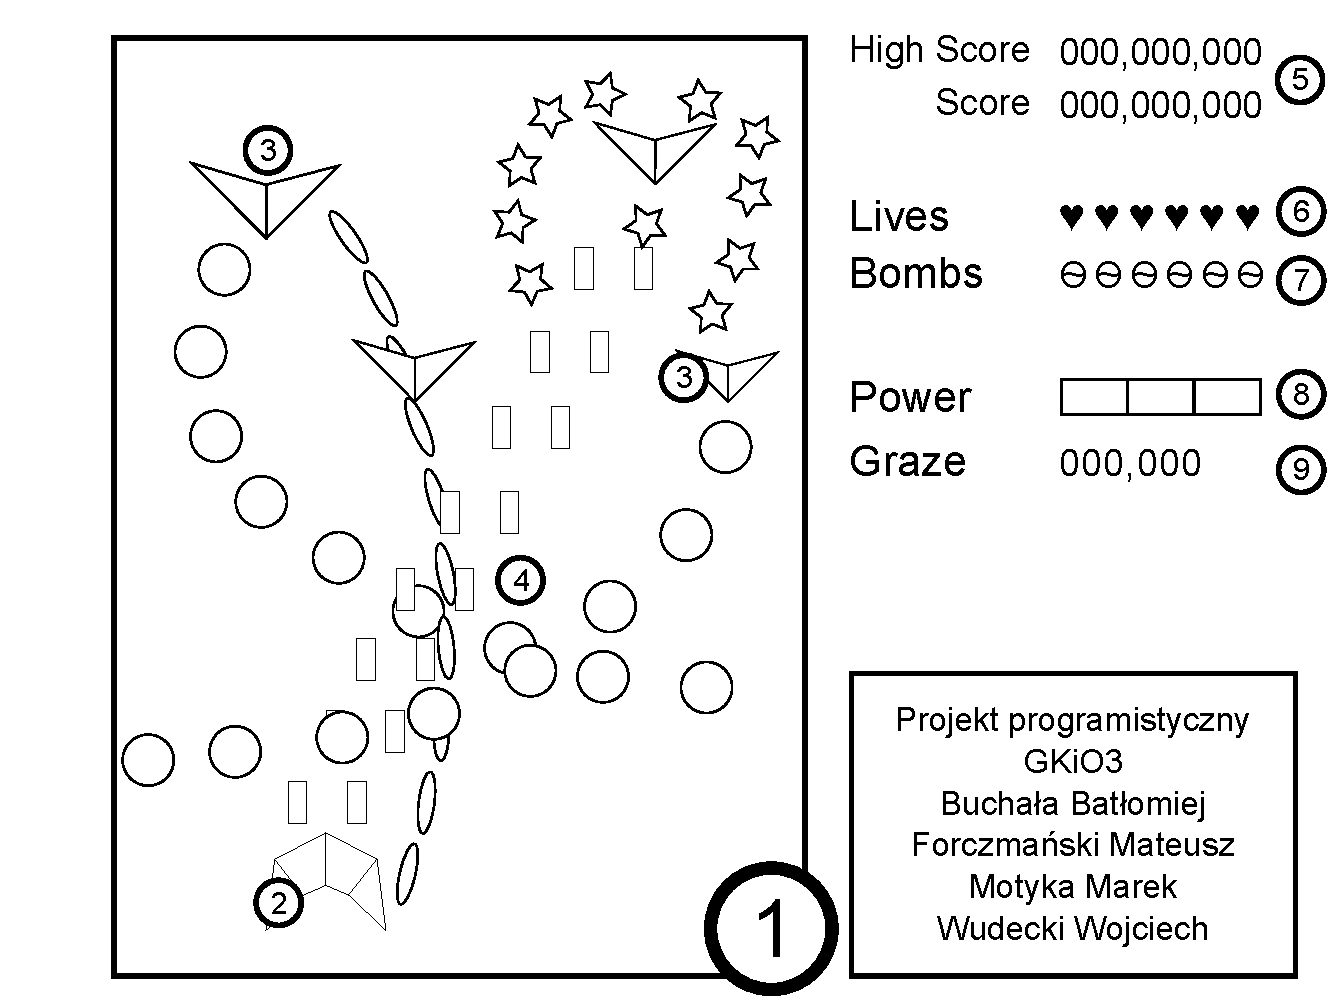
\includegraphics[width=0.8\textwidth]{./images/screen01}%
		}
		\vspace{5pt}
	\end{center}
	\begin{enumerate}
		\item Ekran gry właściwej. W jej obrębie znajduje się gracz, pociski oraz wszyscy wrogowie. 
		\item Grywalna postać, porusza się po ekranie gry, unikając pocisków oraz strzelając do wrogów.
		\item Wrogowie, których należy pokonać.
		\item Chmara pocisków. Jak widać na rysunku, nie wchodzą ze sobą w żadną interakcję, każdy leci swoim wyznaczonym torem. Sprajty wrogów są niewrażliwe na swoje pociski, nie występuje \textit{friendly fire}.
		\item Liczba zdobytych punktów oraz porównywanie ich z największym wynikiem.
		\item Liczba pozostałych żyć. W trakcie gry można zdobywać kolejne. Utrata wszystkich kończy grę.
		\item Liczba pozostałych bomb. Każda wykorzystana bomba zapewnia kilkusekundową odporność na wrogie pociski oraz umożliwia pojedynczy silniejszy atak. Można je zdobyć w trakcie gry.
		\item Pasek mocy, napełnia się w trakcie gry wraz ze zdobytymi punktami. Utrata życia skutkuje zmniejszeniem paska o 1 segment.
		\item Liczba "otarć", czyli uniknięć bardzo blisko pocisku. Aby umożliwić większe wyzwanie, ostateczny wynik pomnożony jest przez licznik Graze.
	\end{enumerate}